\section{Appendix}

We provide an alternative method via circle patterns to obtain
an angle-splitting of the torihedral decomposition
in \secref{s:auglinks}.
This guarantees that the resulting angle structure
on the final triangulation
also satisfies Thurston's gluing equations.
Thus, one can obtian lower bounds on volume
from these angles.


Let $\Gamma$ be a graph on the torus $\torus$,
and let $V,E,F$ be the set of vertices, edges, faces, respectively.
Generally we assume that graphs do not have bigon faces
nor self-loop edges.


$\vec{E}$ is the set of oriented edges.
We may identify an oriented edge $\vec{e}$ with the pair $(f_{\vec{e}}, e)$,
where $f_{\vec{e}}$ is the face to the left of $\vec{e}$.


When we use $\cev{e}$ to refer to an oriented edge, it refers to
the oppositely oriented edge to $\vec{e}$.
If we construct an expression with both $\vec{e}$ and $\cev{e}$,
it will always be (anti-)symmetrical in the two orientations,
and we assume that an arbitrary choice has been made.

%===============================================================================

Recall that a cirlce pattern for a graph $\Gamma$ is an arrangement of circles
in $\torus$ such that each circle circumscribes a face of $\Gamma$.
A circle pattern is determined by the radius of the circle $C_f$ associated to each face, $r_f$,
and the angle that each edge subtends in adjacent faces, $\vphi_{\vec{e}}$.
(See \figref{f:circle_pattern})
\begin{figure}
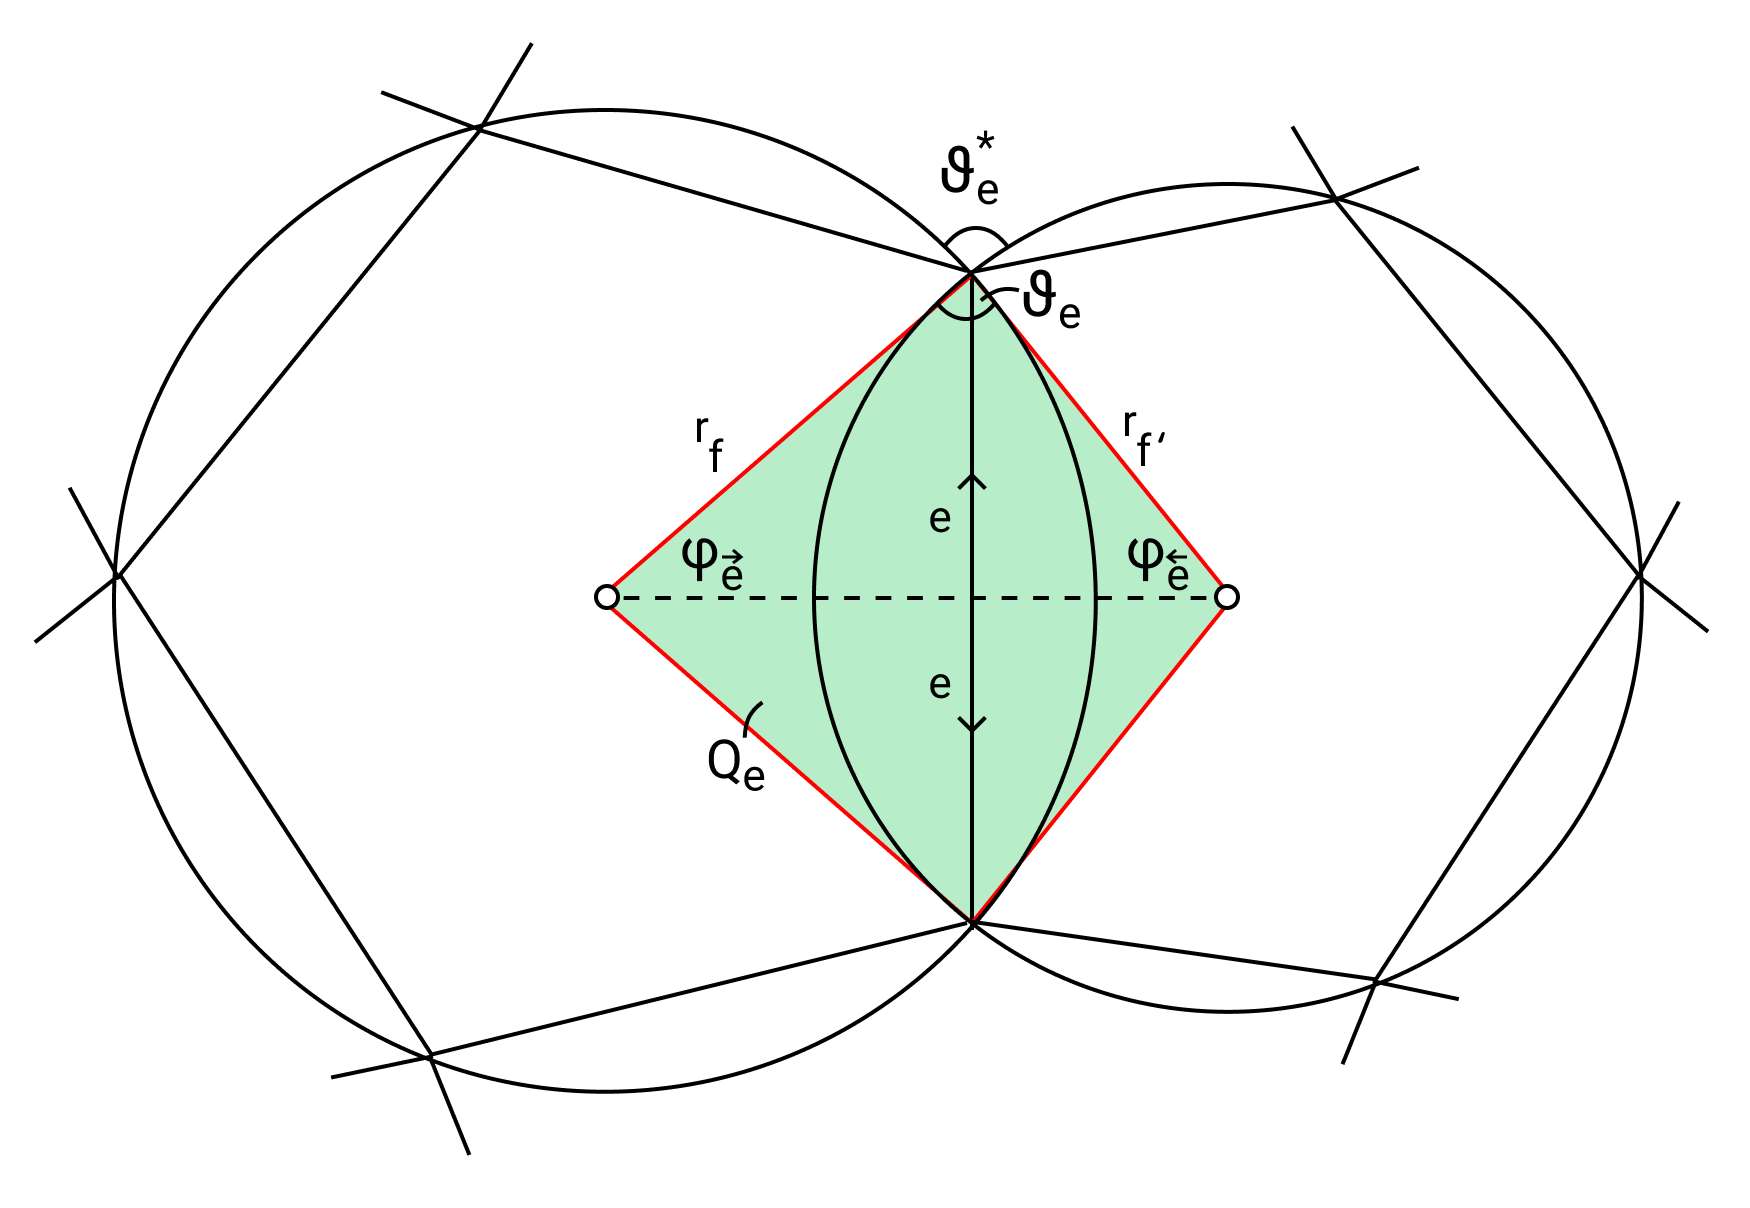
\includegraphics[width=8cm]{circle_pattern}
\caption{Circle pattern in terms of radii $r_f$ and angles $\vphi_{\vec{e}}$}
\label{f:circle_pattern}
\end{figure}
Thus determines, and is determined by a point in $\RRR \times \QQQ$, where

\begin{itemize}
	\item $\RRR := \RR_+^F = \{(r_f)_{f\in F} | r_f \in \RR_+\}$
	\item $\QQQ := \RR^{\vec{E}} =
		\{(\vphi_{\vec{e}})_{\vec{e} \in \vec{E}} | \vphi_{\vec{e}} \in \RR\}$
\end{itemize}
but clearly not every point $c\in \RRR \times \QQQ$ determines a circle pattern.
This larger space allows us to consider
``degenerate" circle patterns, where adjacent circles may
be identical or tangent.


On $\RRR \times \QQQ$, there are several functions to consider:
\begin{itemize}
	\item $\Phi_f = 2 \sum_{\vec{e} \in \del f} \vphi_{\vec{e}}$, measuring the cone angle
		at the center of $C_f$
	\item $\theta_e = \pi - \vphi_{\vec{e}} - \vphi_{\cev{e}}$
	\item $l_{\vec{e}} = 2 r_{f_{\vec{e}}} \sin \vphi_{\vec{e}}$
\end{itemize}

These fit together to give maps to the following spaces:

\begin{itemize}
	\item $\PPP := \RR^F = \{(\Phi_f)_{f\in F} | \Phi_f \in \RR\}$
	\item $\TTT := \RR^E = \{(\theta_e)_{e \in E} | \theta_e \in \RR\}$
	\item $\LLL := \RR^{\vec{E}} = \{(l_{\vec{e}})_{\vec{e} \in E} | l_{\vec{e}} \in \RR\}$
\end{itemize}



\begin{define}
Let $\Gamma$ be a graph on the torus.
An \emph{extended circle pattern} on $\Gamma$ is
$c = ((r_f), (\vphi_{\vec{e}})) \in \RRR \times \QQQ$
such that $l_{\vec{e}} = l_{\cev{e}}$ for all edges $e\in E$. We denote by
$\CCC$ the set of extended circle patterns.
\end{define}



\begin{tikzcd}
\CCC = \{l_{\vec{e}} = l_{\cev{e}} \} \ar[r, "\subset"]
	& \RRR \times \QQQ \ar[r, "\Theta"] \ar[d, "\Phi"]
	& \TTT \\
	& \PPP
\end{tikzcd}


The notion of a circle pattern that is considered in \cite{BandS}
would be restricted to those $c\in \CCC$
with $\vphi_{\vec{e}} \in (0,\pi)$ and $\theta_e \in (0,\pi)$.
They parametrize circle patterns by $(r_f)$ and $(\theta_e)$
(or $(\theta_e^*)$),
and call $(\vphi_{\vec{e}})$ a coherent angle system.
One may consider deforming a circle pattern so as to have
some $\theta_e$ approach 0 or $\pi$.
The limit $\theta_e \to \pi$ is easy to picture, one simply gets that the two circles
$C_f, C_{f'}$ of the adjacent faces become tangent. The limit $\theta_e \to 0$
is a bit more complex, as the final shape of $Q_e$ (the quadrangle associated to $e$)
may depend on $\vphi_{\vec{e}}$ or $\vphi_{\cev{e}}$.
If we parametrize circle patterns by $(r_f)$ and $(\theta_e)$ as in \cite{BandS},
the limiting shape would depend on the relationship between 
$r_f$ and $r_{f'}$.
As our main result depends on extending \cite{BandS} result
to such limits and beyond,
we find it more convenient to describe extended circle patterns by
$(r_f)$ and $(\vphi_{\vec{e}})$.


We will mostly be working with extended circle patterns that ``look normal'',
with all $\vphi_{\vec{e}}$ in the range $[0,\pi)$,
so we do not dwell on the meaning of negative $\vphi_{\vec{e}}$'s.
\footnote{
Intuitively, one can visualize decreasing $\vphi_{\vec{e}}$
from $\veps$ to $-\veps$
as moving the black vertices of the quadrangle $Q_e$ past each other,
thus flipping $Q_e$ along its long axis
and making it have negative area.
}

\begin{define}
An extended circle pattern is said to be \emph{face non-singular}
if $\Phi_f = 2\pi$ for all faces $f$; it is said to be \emph{vertex non-singular}
if $\sum_{e \ni v} \theta_e = 2\pi$ for all vertices $v$.
Finally it is said to be \emph{non-singular} if it is both.
\end{define}


\begin{define}
Let $f$ be a non-singular face (i.e. $\Phi_f = 2\pi$),
such that for all edges $\vec{e} \in \del f$,
$\vphi_{\vec{e}} \in [0,\pi)$.
We say $f$ is \emph{thin} if
exactly two edges of $f$ have nonzero $\vphi_\bullet$;
we say it is \emph{thick} otherwise.
We say it is \emph{convex} if for all edges $\vec{e} \in \del f$,
we have $\vphi_{\vec{e}} \in [0,\pi/2)$.
\end{define}


%\begin{define}
%Given some extended circle pattern $c \in \CCC$,
%we say a face $f$ is \emph{convex} if for all edges $\vec{e} \in \del f$,
%we have $\vphi_{\vec{e}} \in [0,\pi/2)$.
%We say $f$ is \emph{thin} if exactly two edges $\vec{e}, \vec{e'} \in \del f$
%have nonzero $\vphi_{\bullet}$, and furtheremore,
%	$0 < \vphi_{\vec{e}} = \pi - \vphi_{\vec{e'}} < \pi/2$.
%\end{define}

%figures for convex, thin faces

\begin{define}
Given an extended circle pattern $c\in \CCC$, an edge $e$ is \emph{short}
if it has length 0, $l_e = 0$;
it is \emph{long} otherwise.
\end{define}


\begin{define}
Given an extended circle pattern $c\in \CCC$, a \emph{wide path}
is a sequence of faces $f_0,f_1,\ldots,f_n$
such that $f_i,f_{i+1}$ share a long edge.
A \emph{wide cycle} is a wide path with $f_0 = f_n$.
\end{define}


\begin{lemma}
\label{l:manifold_point}
Let $c$ be a face non-singular extended circular pattern
such that $\vphi_{\vec{e}} \geq 0$ for all $\vec{e}\in\vec{E}$.
Furthermore, suppose that there is no cycle of edges
$e_0, e_1, \ldots, e_n = e_0$ such that
$e_i, e_{i+1}$ belong to the same face,
and $\vphi_{\vec{e_i}} = \vphi_{\cev{e_i}} = \pi/2$.
Then $\CCC$ is a manifold in a neighborhood of $c$.
\end{lemma}
\begin{proof}
We need to show that the differentials
$d(l_{\vec{e}} - l_{\cev{e}})
= 2\sin \vphi_{\vec{e}} d r_{f_{\vec{e}}}
+ 2r_{f_{\vec{e}}} \cos \vphi_{\vec{e}} d \vphi_{\vec{e}}
- 2\sin \vphi_{\cev{e}} d r_{f_{\cev{e}}}
- 2r_{f_{\cev{e}}} \cos \vphi_{\cev{e}} d \vphi_{\cev{e}}
$
are linearly independent at $c$.
If $\vphi_{\vec{e}} \neq \pi/2$,
then the $d\vphi_{\vec{e}}$ term makes $d(l_{\vec{e}} - l_{\cev{e}})$
linearly independent from the rest
(no other differential $d(l_{\vec{e'}} - l_{\cev{e'}})$
contains such component);
likewise for $\vphi_{\cev{e}} \neq \pi/2$.


Now consider the set $E'$ of edges $e$ that have
$\vphi_{\vec{e}} = \vphi_{\cev{e}} = \pi/2$.
Consider a maximal sequence of faces $f_0,\ldots,f_n$
with no repetitions and $f_i,f_{i+1}$ share
an edge $e_i \in E'$.
By the condition on no cycles,
$f_0 \neq f_n$.
By face non-singularity, any face can meet at most two
edges from $E'$, thus if $e\in E'$,
it is contained in a unique such string of faces/edges.
Thus the differentials
$d(l_{\vec{e_i}} - l_{\cev{e_i}}) = 2dr_{f_i} - 2dr_{f_{i+1}}$
are linearly independent.
\end{proof}



\subsection{From Extended Circle Patterns to Hyperbolic Polyhedra}
In this section, we describe how to obtain a
decomposition of a torihedron into hyperbolic ideal pyramids
from a non-singular extended circle pattern.

\begin{lemma}
\label{l:circpattern_polyhedra}
Suppose we have the graph of a torihedron.
Given a non-singular extended circle pattern $c \in \CCC$ on the graph,
such that all $\vphi_{\vec{e}} \in (0,\pi)$,
there exists a decomposition of the torihedron
into base-angled ideal pyramids such that
	\begin{itemize}
		\item each interior edge of the torihedron has dihedral angles sum to $2\pi$;
		\item each boundary edge $e$ of the torihedron has dihedral angles sum to
			$\pi - \theta_e$.
	\end{itemize}
\end{lemma}

\begin{proof}
For each directed edge $\vec{e} \in \vec{E}$,
construct the isosceles triangle $T_{\vec{e}}$
with equal sides of length $r_{f_{\vec{e}}}$ and
angle $2\tilde{\vphi}_{\vec{e}}$ subtended between them,
where $\tilde{\vphi}_{\vec{e}} = \vphi_{\vec{e}}$
if $\vphi_{\vec{e}}$ if it is acute,
and = $\pi - \vphi_{\vec{e}}$ otherwise.

\begin{figure}
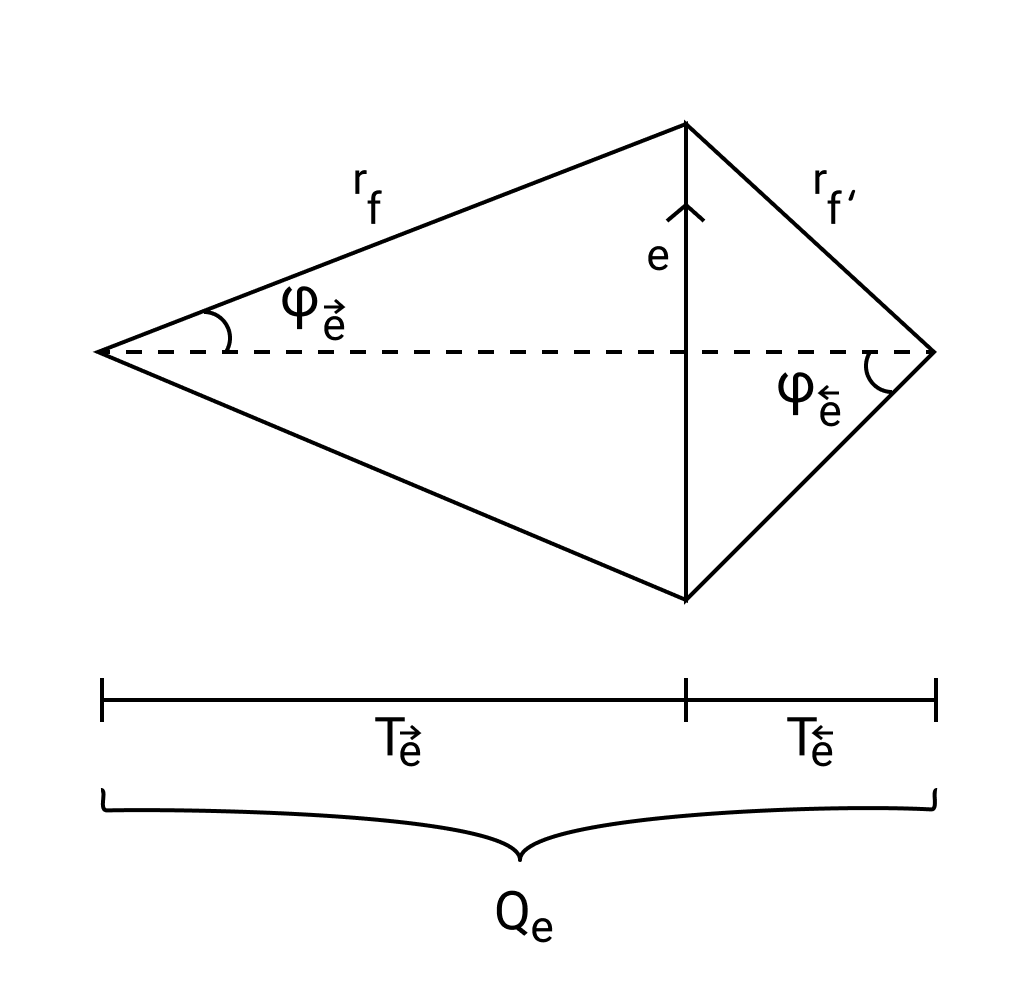
\includegraphics[width=8cm]{more_pictures/kite.png}
	\caption{The kite of two circles intersecting in a ``normal" circle pattern.}
\end{figure}
\begin{figure}
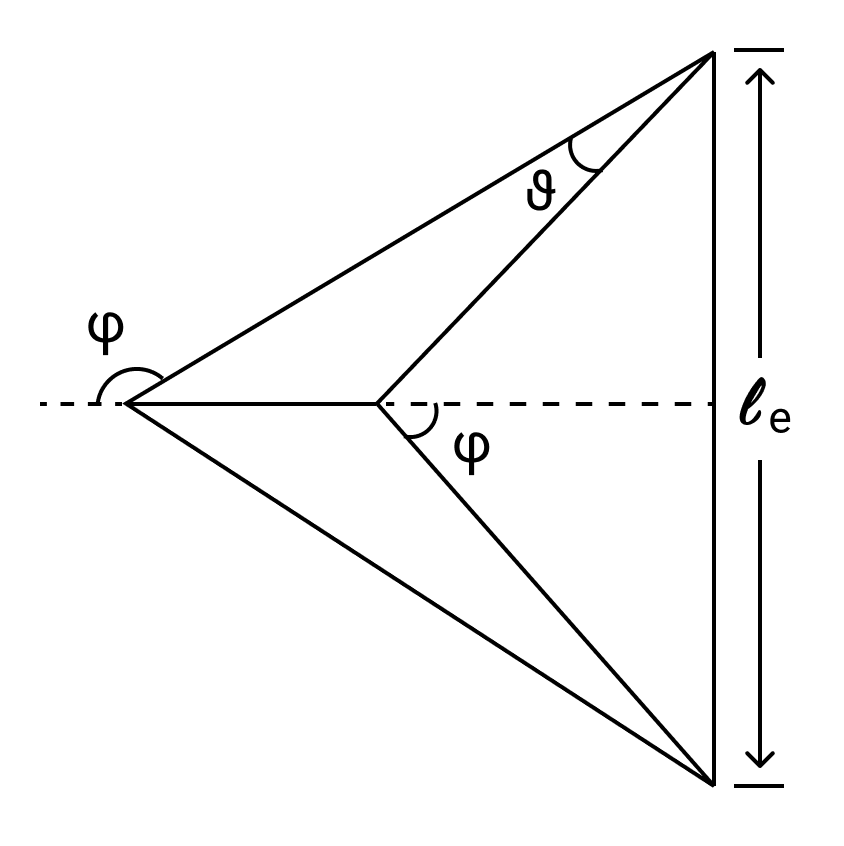
\includegraphics[width=5cm]{more_pictures/positive_angle.png}
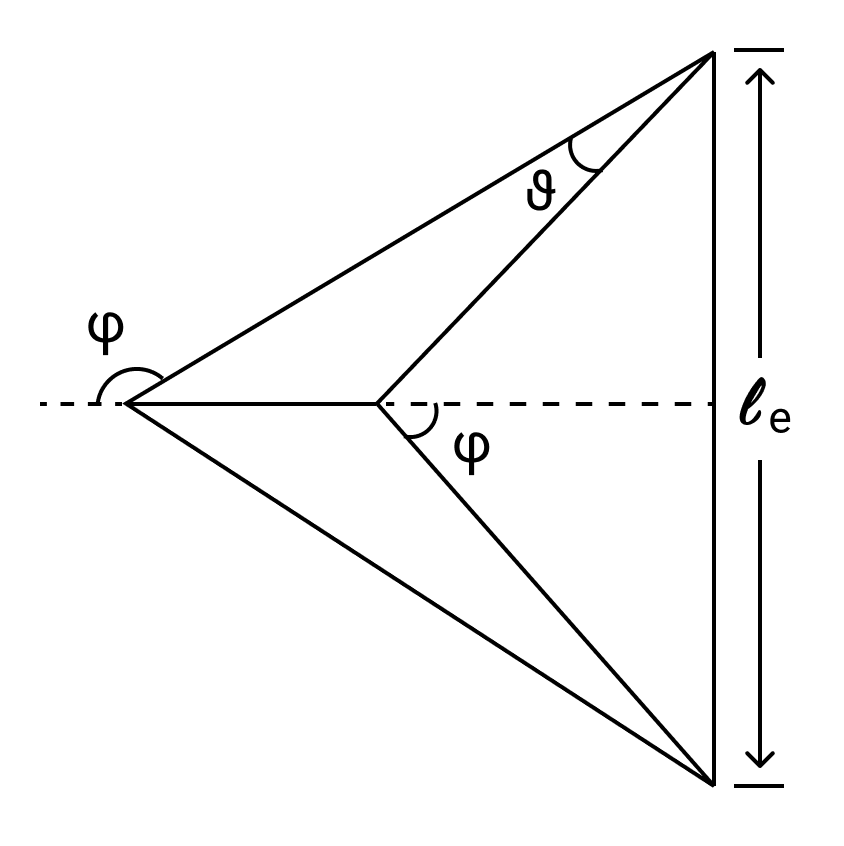
\includegraphics[width=5cm]{more_pictures/negative_angle.png}
	\caption{Kites of a degenerate circle pattern.}
\end{figure}


Let $f \in F$ be a face.
We construct a Euclidean polygon $\Pol_f$ as follows.
If $\vphi_{\vec{e}} \leq \pi/2$ for all $\vec{e} \in \del f$,
i.e. if $f$ is convex, then 
the $T_{\vec{e}}$ for $\vec{e}\in \del f$
fit together into $\Pol_f$.
If not, suppose $\vphi_{\vec{e}} > \pi/2$
for $\vec{e} = \vec{e_1}$, 
and $\leq \pi/2$ for $\vec{e} = \vec{e_2},\ldots \vec{e_k} \in \del f$.
Then put $T_{\vec{e_2}},\ldots,T_{\vec{e_k}}$ together as above,
creating a $(k+1)$-gon,
then subtract $T_{\vec{e_1}}$ from it to form $\Pol_f$.

Thus, to each face, we associate the Euclidean polygon $\Pol_f$.
If $v$ is the vertex of $\Pol_f$ between $e_i$ and $e_{i+1}$,
then the angle at $v$ is
$\pi - \vphi_{\vec{e_i}} - \vphi_{\vec{e_{i+1}}}$.
Then the non-vertex-singularity of $c$ guarantees that
the sum of angles at $v$ of $\Pol_f$, for faces $f$ containing $v$,
is $2\pi$.
%; in other words, $\Pol_f$ glue along edges


View the Euclidean plane as the boundary of the upper-half space.
Then $\Pol_f$ supports an ideal hyperbolic pyramid $P_f$.

Clearly, these $P_f$'s, as abstract ideal tetrahedra,
glue together into the torihedron.
%The hyperbolic structure on $P_f$
%in particular provide dihedral angles to each edge of $P_f$
%which clearly satisfies the conditions of making $P_f$
%a base-angled ideal pyramid.
We need to check that the angles around each edge of
the torihedron have the appropriate angles.


Consider an interior edge $e$ of the pyramidal decomposition
of the torihedron.
It corresponds to a vertex $v$ of the graph.
Note that the dihedral angle of the vertical edge
at $v$ of $P_f$ is simply the angle at $v$ of $\Pol_f$;
these sum to $2\pi$ over $f \ni v$.


For a boundary edge $e$, the dihedral angles at $e$ of the $P_f$'s
containing it are $\vphi_{\vec{e}}$ and $\vphi_{\cev{e}}$,
which sum to $\theta_e$ by definition.

\end{proof}


\subsection{Deforming Extended Circle Patterns}



Our general strategry for obtaining a (non-singular) circle pattern
is to start with an assignment $\underline{\theta} = (\theta_\bullet)$
for which we know an extended circle pattern exists
(say from results of \cite{BandS}),
and a path $\gamma$ in $\TTT$ starting at $\underline{\theta}$.
We then attempt to lift $\gamma$ to a path $\tilde{\gamma}$ in $\CCC$,
so that $\tilde{\gamma}$ remains (face) non-singular
(vertex non-singularity is already determined by $\gamma$).

Note that since $\sum_{e\in E} \theta_e
= 2\pi |E| - \sum_{\vec{e} \in \vec{E}} \vphi_{\vec{e}}
= 2\pi |E| - \sum_{f\in F} \Phi_f$,
we see that maintaining face non-singularity of $\tilde{\gamma}$
forces $\sum \theta_e$ to be constant.
We will show that this is the only obstruction on $\gamma$
to the lifting to such $\tilde{\gamma}$.

To that end, let $L$ be the $(|E|-1)$-plane distribution on $\TTT$
tangent to the level sets of $\sum_{e\in E} \theta_e$.
The following proposition proves that we can deform
some circle patterns up to first order at a point:


\begin{prop}
\label{p:point_lift}
Let $c \in \CCC$ be a
non-singular extended circle pattern on a graph
with no bigons or self-loops such that
there is no wide cycle of thin faces,
and each edge meets two distinct faces.
Let $K_c = \ker (\Phi_*|_c : T_c \CCC \to T_{\Phi(c)} \PPP)$.
Then $\Theta_*(K_c) = L_{\Theta(c)}$.

In other words, for any vector $a \in T_{\Theta(c)} \TTT$
with sum of components 0, one can vary $c$ so that its
first order change in $\theta_\bullet$ is $a$,
and also remains face non-singular up to first order.
\end{prop}


Before we prove this, it is convenient to first prove the following,
which will establish some useful notation:

\begin{lemma}
\label{l:Phi_full}
Let $c \in \CCC$ be as in \prpref{p:point_lift}.
Then $\Phi$ is a submersion in a neighbourhood of $c$.
\end{lemma}

\begin{proof}
We construct vectors $\beta_f \in T_c \CCC$ so that
$\Phi_*(\beta_f) = \ddd{\Phi_f}$.
The vector
\begin{equation}
\label{e:alpha_f}
\alpha_f := \ddd{r_f} - \sum_{\vec{e} \in \del f} 
	\frac{\tan \vphi_{\vec{e}}}{r_f} \ddd{\vphi_{\vec{e}}}
	\in T(\RRR \times \QQQ)
\end{equation}
doesn't change $l_{\vec{e}}$,
so is in $T_c \CCC$.
Intuitively, $\alpha_f$ is like
pulling the center of $C_f$ up off the plane, increasing $r_f$ and decreasing all
$\vphi$'s.
Its pushforward under $\Phi$ is simply
$\Phi_*(\alpha_f) =
	(-\frac{2}{r_f} \sum_{\vec{e}\in \del f} \tan \vphi_{\vec{e}})
	\ddd{\Phi_f}$.


If $f$ is a convex face, then the $\tan \vphi_{\vec{e}}$ are all non-negative,
being 0 if and only if $e$ is short,
and because $\Phi_f = 2\pi$, at least three edges are long.
So $\Phi_*(\alpha_f)$ is a negative multiple of $\ddd{\Phi_f}$;
we choose $\beta$ so that
\begin{equation}
\label{e:beta_f_convex}
\beta_f := \beta \cdot \alpha_f; \;\;\;
\Phi_*(\beta_f) = \ddd{\Phi_f}
\end{equation}

If $f$ is thick but not convex,
let $\vec{e}$ be an edge with largest $\vphi_{\vec{e}}$,
so that $\vphi_{\vec{e}} \geq \pi/2$.
If $\vphi_{\vec{e}} > \pi/2$,
then since $\tan$ is convex, and $f$ has at least two other
long edges,
we see that $\Phi_*(\alpha_f) = -\sum \frac{\tan \vphi_{\vec{e'}}}{r_f} > 0$,
so we can define $\beta_f$ as in \eqnref{e:beta_f_convex}.
If $\vphi_{\vec{e}} = \pi/2$,
we can take
\[
\beta_f = \frac{1}{2} \ddd{\vphi_{\vec{e}}}
\]



If $f$ is thin, we actually have that $\alpha_f \in K_c$,
since the components sum to 0, so we need a different approach.
First suppose $f$ shares an edge $e$ with a thick face $f'$,
with $\vec{e} \in \del f$.
If $\vphi_{\vec{e}} = \pi/2$, we can take
$\beta_f = \frac{1}{2} \ddd{\vphi_{\vec{e}}}$ as before.
Otherwise, we can increase $l_{\vec{e}}$
by varying $\vphi_{\vec{e}}$
while holding $r_f$ constant,
and increase $l_{\cev{e}}$
by increasing $r_{f'}$.
This will affect both $\Phi_f, \Phi_{f'}$,
so we use $\beta_{f'}$ to make $\Phi_{f'}$ constant.
%More explicitly, consider
%\begin{equation}
%\label{e:alpha_e}
%\alpha_e = \frac{1}{2 r_f \cos \vphi_{\vec{e}}} \ddd{\vphi_{\vec{e}}}
%+ \frac{1}{2 r_{f'}\cos \vphi_{\cev{e}}} \ddd{\vphi_{\cev{e}}}
%\end{equation}
%which increases $l_{\vec{e}}, l_{\cev{e}}$ at half unit speed,
%$dl_{\vec{e}}(\alpha_e) = dl_{\cev{e}}(\alpha_e) = 1/2$.
%Then we can take
%\begin{equation}
%\label{e:beta_f_thin}
%\beta_f = r_f \cos \vphi_{\vec{e}}
	%(\alpha_e - \frac{1}{r_{f'} \cos \vphi_{\cev{e}}} \beta_{f'})
%\end{equation}
We can repeat this procedure with $f'$ set to this thin face,
and $f$ set to another thin face adjacent to it, etc.
\end{proof}

\begin{proof}
We construct a vector $u_e \in K_c \subseteq T_c \CCC$ for each edge $e$
and show that $\{\Theta_*(u_e)\}_{e\in E}$ spans an
$|E|-1$ dimensional space,
thus must be equal $L_{\Theta_c}$.
The vectors $u_e$ will have the following property:
if $\Theta_*(u_e) = \sum_{e' \in E} a^{e'} \ddd{\theta_{e'}}$, then
\begin{itemize}
	\item $a^e = 1$;
	\item $a^{e'} \leq 0$ for all $e' \neq e$;
	%\item $a^{e'} = 0$ for short edges $e'$ (hmm...)
	\item $\sum_{e' \in E} a^{e'} = 0$ (follows directly from $u_e \in K_c$)
\end{itemize}

Furthermore, these $u_e$'s collectively satisfy the following
connectivity property:
consider the graph $G$ whose vertex set is the set of edges $E$,
and we connect two long edges $e,e'$ by an edge if there is some $e''$ such that
$a^e, a^{e'}$ are both nonzero in $\Theta_*(u_{e''})$;
then $G$ is connected.


Let us first suppose we have constructed such $u_e$,
and show that these properties ensure that
$\{\Theta_*(u_e)\}_{e\in E}$ spans an $|E|-1$ dimensional space.
This is a simple exercise in linear algebra,
but we show it for completeness.


Put the $\Theta_*(u_e)$'s into a $E \times E$ matrix,
denoted $M$,
so that the $e$-th row corresponds to $\Theta_*(u_e)$.
By virtue of $u_e \in K_c$, we have that $(1\; 1\; \cdots \; 1)^T$
is in the null space of $M$;
our goal is to show that it spans the null space.


Suppose $b = (b_e)^T$ is in the null space of $M$.
Let $|b_e|$ be the largest among components of $b$;
rescale $b$ so that $b_e = 1$.
The $e$-th component of $M b$
is $1 - \sum_{e' \neq e} a^{e'} b_{e'}$,
where $a^{e'}$ are the components of $\Theta_*(u_e)$.
Since $\sum_{e' \neq e} |a^{e'}| = 1$, this can be 0 if and only if
for all $e'$ with $a^{e'} < 0$, we have exactly $b_{e'} = 1$.
We then repeat this argument on the other $e'$
that appear in $\Theta_*(u_e)$.
By connectedness of $G$, this implies
$b = (1 \; \cdots \; 1)^T$,
thus $M$ has rank $|E|-1$.


Before constructing the $u_e$'s,
let us first construct several other auxiliary vectors
that are not necessarily in $T_c \CCC$.
Generally they keep $\Phi_f$'s constant,
but have an effect on the lengths of oriented edges $l_{\vec{e}}$.
The $u_e$'s will be built from a combination of these.
All discussion of changes will refer to changes in the first order.


Let $f$ be a convex face, and $\vec{e} \in \del f$. Define
\begin{equation}
\label{e:eta_e}
\eta_{\vec{e}} =
\frac{1}{2 r_f \cos \vphi_{\vec{e}}} \ddd{\vphi_{\vec{e}}}
- \frac{1}{r_f \cos \vphi_{\vec{e}}} \beta_f
\end{equation}
$\eta_{\vec{e}}$ keeps $\Phi_f$ constant, but increases $l_{\vec{e}}$
at unit speed, i.e. $dl_{\vec{e}}(\eta_{\vec{e}}) = 1$.


Let $f$ be a thick but not convex face.
There is exactly one edge $\vec{e} \in \del f$
with $\vphi_{\vec{e}} \geq \pi/2$.
If $\vphi_{\vec{e}} > \pi/2$, we will define
$\eta_{\vec{e}}$ as in \eqnref{e:eta_e}.
If $\vphi_{\vec{e}} = \pi/2$,
we will define
\begin{equation}
\label{e:eta_e_2}
\eta_{\vec{e}} = \frac{1}{2}\ddd{r_f}
+ \big(\sum_{\vec{e'} \neq \vec{e}}
	\frac{\sin \vphi_{\vec{e'}}}{2 r_f \cos \vphi_{\vec{e'}}}\big)
	\ddd{\vphi_{\vec{e}}}
- \sum_{\vec{e'} \neq \vec{e}}
	\frac{\sin \vphi_{\vec{e'}}}{2 r_f \cos \vphi_{\vec{e'}}}
	\ddd{\vphi_{\vec{e'}}}
\end{equation}
Then it is easy to see that
$dl_{\vec{e}}(\eta_{\vec{e}}) = 1$
while
$dl_{\vec{e'}}(\eta_{\vec{e}}) = 0$
for all other $\vec{e'} \neq \vec{e}$,
and $\eta_{\vec{e}}$ keeps $\Phi_f$ constant.


Now let $\vec{e'} \in \del f$ be another edge.
We define
\begin{equation}
\label{e:gamma_e}
\gamma_{\vec{e'}} = \frac{1}{2 r_f \cos{\vphi_{\vec{e'}}}}
	(\ddd{\vphi_{\vec{e'}}} - \ddd{\vphi_{\vec{e}}})
\end{equation}
Then $dl_{\vec{e'}} = 1$,
$dl_{\vec{e}} = -\frac{\cos \vphi_{\vec{e}}}{\cos \vphi_{\vec{e'}}} \geq 0$,
and keeps $\Phi_f$ constant.


Finally, let $f$ be a thin face.
If $\vec{e} \in \del f$ is a short edge,
i.e. $\vphi_{\vec{e}} = 0$,
then we define $\eta_{\vec{e}}$ as in \eqnref{e:eta_e}.
If $\vec{e}$ is long, and $\vphi_{\vec{e}} \neq \pi/2$,
we define $\gamma_{\vec{e}}$ as in \eqnref{e:gamma_e};
if $\vphi_{\vec{e}} = \pi/2$, we define
\begin{equation}
\label{e:xi_e}
\xi_{\vec{e}} = \frac{1}{2}\ddd{r_f}
\end{equation}
Clearly $dl_{\vec{e}}(\xi_{\vec{e}}) = dl_{\vec{e'}}(\xi_{\vec{e}}) = 1$
for the other edge $e'$ with $\vphi_{\vec{e'}} = \pi/2$.
%where $\vec{e'} \in \del f$ is the unique other long edge.


In summary,
$\eta_{\vec{e}}, \gamma_{\vec{e}}, \xi_{\vec{e}}$
always increases $l_{\vec{e}}$ at unit speed,
and keeps $\Phi_{f_{\vec{e}}}$ constant.
$\eta_{\vec{e}}$ does not affect the lenghts of other edges
in the face $f_{\vec{e}}$,
but the other two might affect another edge
- this other edge $\vec{e'}$ is unique,
and $l_{\vec{e}}, l_{\vec{e'}}$ either both increase
or decrease.
Furthermore, $l_{\vec{e'}} \geq l_{\vec{e'}}$.


For any oriented edge $\vec{e}$,
there is exactly one such vector defined for it;
call that vector $\zeta_{\vec{e}}$.


Now we can put these vectors together to construct the desired $u_e$'s.
To illustrate the main idea of the construction,
first suppose that $e$ is an edge between two convex faces $f,f'$.
Then we can consider
\[
w_e = \eta_{\vec{e}} + \eta_{\cev{e}}
\]
Since $dl_{\vec{e}}(w_e) = dl_{\cev{e}}(w_e) = 1$,
and $dl_{\vec{e'}}(w_e) = 0$ for all other edges,
$w_e \in T_c \CCC$;
furthermore, $\eta_-$ does not affect $\Phi_-$,
so $w_e \in K_c$.
For $\vec{e'} \in \del f \cup \del f' \backslash \{\vec{e},\cev{e}\}$,
the $\ddd{\vphi_{\vec{e'}}}$ component only appears in $\beta_f$
or $\beta_{f'}$, which is positive by construciton
(because $f,f'$ are convex faces);
thus, $d\theta_{e'}(w_e) \geq 0$ for such $e'$, and
is equal to 0 if and only if $e'$ is short.
Finally, since $w_e \in K_c$, it leaves the sum $\sum_{e\in E} \theta_e$
constant, so $d\theta_e(w_e) < 0$, so we can take
\begin{equation}
\label{e:u_e}
u_e := (d\theta_e(w_e))^\inv \cdot w_e
\end{equation}


Now consider an arbitrary edge $e$ between faces $f,f'$.
We build $u_e$ inductively, beginning with
$w_e = \zeta_{\vec{e}} + \zeta_{\cev{e}}$,
$F' = \{f, f'\}$, and $E' = \{e\}$.
If $w_e$ also affects $l_{\vec{e'}}$ for some edge
$\vec{e'} \in \del F' \backslash\{\vec{e''},\cev{e''} | e''\in E'\}$,
we add an appriopriate positive multiple
of $\zeta_{\cev{e'}}$ to $w_e$,
add $f_{\cev{e'}}$ to $F'$,
and add $e'$ to $E'$.
Recall that when $\zeta_{\vec{e'}}$ affects
the length of another edge $e''$,
we always have $l_{\vec{e''}} \geq l_{\vec{e'}}$.
Thus by the condition of non-existence of wide cycles of thin faces,
this process must terminate.
It is not hard to see that when an $\eta_-$ term appears,
the process terminates (for that direction);
a $\gamma_-$ term begets either another $\gamma_-$ or $\eta_-$ term;
a $\xi_-$ term begets either
a $\xi_-, \gamma_-$, or $\eta_-$ term.
In other words, in the end we get some sum
(ignoring possible positive coefficients)
\[
w_e = (\xi_- + \xi_- + \cdots + \gamma_- + \gamma_- + \cdots + \eta_-)
+ (\xi_- + \xi_- + \cdots + \gamma_- + \gamma_- + \cdots + \eta_-)
\]
where in each parenthesis,
the first term affects the next term and so on.


Assume that there are no thin faces.
We check that $w_e$ has the desired properties.
By construction, $w_e \in T_c \CCC$.
Observe that the coefficient of $\ddd{\vphi_{\vec{e}}}$
is positive in either $\eta_{\vec{e}}$ or $\gamma_{\vec{e}}$,
so $d\theta_e(\Theta_*(w_e)) < 0$.
There is a maximal sequence of thick faces
$f_0 = f, f_1, \ldots, f_n$
and a sequence of edges $e_0 = e, e_1, \ldots, e_n$,
where for $i\neq 0$, $e_i$ is between $f_{i-1}$ and $f_i$,
and $l_{e_i}$ increases under $w_e$;
we label oriented edges so $\vec{e_i} \in \del f_i$,
$\cev{e_i} \in \del f_{i+1}$.
(Similar discussion for $f_0 = f'$).
Consider one of the edges $e_i$, $i\neq 0$.
Since $l_{e_i}$ increases, the $\zeta_{\vec{e}_{i-1}}$ term
from the previous edge $e_{i-1}$ must have been
$\gamma_{\vec{e}_{i-1}}$;
in particular, $\vphi_{\cev{e_i}} > \pi/2$,
$w_e$ decreases $\vphi_{\cev{e_i}}$,
and keeps $r_{f_{i-1}}$ constant.
The edge $e_i$ also contributes some $\zeta_{\vec{e_i}}$
term to $w_e$;
it increases $\vphi_{\vec{e_i}}$ and either increases
or keeps constant $r_{f_i}$.
Then $\theta_{e_i}$ increases, i.e. $d\theta_{e_i}(\Theta_*(w_e)) > 0$,
by the following simple exercise in elementary Euclidean geometry.
Suppose an obtuse triangle $\triangle ABC$, $\angle B > \pi/2$,
and we decrease $\angle B$, increase $\angle C$,
keep length of $\overline{AB}$ constant,
and either increase or keeps constant the length of $\overline{AC}$;
then $\angle A$ increases.
This can be proved by observing that the changes we are forcing
on the triangle can be broken in two:
the first is increase $\angle B$ and keeping lengths
$\overline{AB}, \overline{AC}$ constant,
and the second is keeping $\angle B$ and length $\overline{AB}$ constant,
and increasing length $\overline{AC}$;
each of these increases $\angle A$.
We apply this to our situation with $B,C$ being
the centers of circles $C_{f_{i-1}}, C_{f_i}$
of the faces $f_{i-1}, f_i$.
As before, we simply rescale $w_e$ appropriately to obtain $u_e$.

Now we consider the presence of thin faces.
If all the $\zeta_-$ terms added to $w_e$
are $\eta_-$ or $\gamma_-$,
then all arguments in the previous paragraph applies.
The only situation in which $\xi_-$ is used
is when either $\zeta_{\vec{e}}$ or $\zeta_{\cev{e}}$ is $\xi_-$.
Without loss of generality, $\zeta_{\vec{e}} = \xi_{\vec{e}}$,
so that $\vec{e} \in \del f$, $f$ is a thin face with nonzero
angles equal to $\pi/2$;
let $\vec{e'}$ be the other edge with $\vphi$ angle $\pi/2$.
Suppose the next face, the one adjacent to $e'$, is not thin.
We simply add $\alpha \cdot (\ddd{\vec{e}} - \ddd{\vec{e'}})$
to $w_e$,
where $\alpha > 0$ is chosen small enough so that, in combination
with the next $w_e$ term $\zeta_{\cev{e'}}$,
$\theta_{e'}$ increases;
for example, if the next term is $\zeta_{\cev{e'}} = \gamma_{\cev{e'}}$,
then we choose $\alpha < \frac{1}{2r \cos \vphi_{\cev{e'}}}$,
the coefficient of $\ddd{\vphi_{\cev{e'}}}$ in $\gamma_{\cev{e'}}$.
If the next face is also thin,
we add the same term, and so on, until we reach a non-thin face.
It is straighforward to check that $\theta_e$ decreases,
and all other affected $\theta_-$'s increase.
\end{proof}



\begin{prop}
\label{p:nghd_lift}
Let $c\in \CCC$ be as in \prpref{p:point_lift}.
Given a smooth path $\gamma: [0,\infty) \to \TTT$
starting at $\gamma(0) = \Theta(c)$
and has constant value $(\sum \theta_e) \circ \gamma$,
there exists $\veps > 0$ and a lift $\tilde{\gamma} :[0, \veps] \to \CCC$
of $\gamma|_{[0,\veps]}$ along $\Theta$
that starts at $\tilde{\gamma}(0) = c$
and has constant value $\Phi \circ \tilde{\gamma}$.
\end{prop}


\begin{proof}
By \lemref{l:Phi_full}, $\Phi$ is a submersion at $c$,
hence is a submersion in a neighborhood $U \in \CCC$ of $c$.
Thus, the kernels
$K_{c'} = \ker(\Phi_*|{c'} : T_{c'} \CCC \to T_{\Phi(c')} \PPP)$
form an $|E|$-plane distribution $K \subset T\CCC|_U$ over $U$.
By \prpref{p:point_lift}, the bundle map
$\Theta_*|_K : K \to L$ is full rank at $c$,
hence it is full in a possibly smaller neighborhood,
which we redefine $U$ to be.


Since $\sum_{e \in E} \theta_e = 2\pi |E| - \sum_{f\in F} \Phi_f$,
the fullness of $\Phi_*$ also shows that
$\sum \theta$ has no critical points in $U$;
for $s$ in some small interval around $(\sum \theta)(c)$,
denote, by overloading notation,
$L_s = (\sum \theta)^\inv (s)$,
$U_s = U \cap \Theta^\inv(L_s)$.
We may consider $K$ as a family of $|E|$-plane distributions
$K_s$ over $U_s$.


The vector $\rho := \sum_{f\in F} r_f \ddd{r_f}$ corresponds to
scaling all radii by the same factor, and is clearly in $T\CCC$.
It is obviously mapped to zero under $\Phi_*$ and $\Theta_*$,
so $\Span\{\rho\} = \ker(\Theta_*|_K) \subset K$.
Thus, over $U$, we may split
$K = \Span\{\rho\} \oplus K'$
(say as orthogonal decomposition w.r.t. some smooth metric on $\CCC$),
so that $\Theta_*|{c'} : K'|_{c'} \simeq L_{\Theta(c')}$.


In other words, $K'|_{U_s}$ is a horizontal $(|E|-1)$-plane distribution
that determines an Ehresmann connection of the
fibre bundle $U_s \to L_s$ (after being appropriately restricted).
Therefore, a short path $\gamma$ starting at $\Theta(c)$
with constant $\sum \theta$, i.e. a path in $L_s$, $s ={(\sum \theta)(c)}$,
can be lifted to a path $\tilde{\gamma}$ in $U_s$,
so that $\tilde{\gamma}$ is always tangent to $K'$,
hence $\Phi(\tilde{\gamma})$ is constant.
\end{proof}


Finally let us say a few words in relation to the proof of hyperbolicity
of augmented links, i.e. the proof of
\thmref{t:auglink_hyp}.
Using Theorem 4 from \cite{BandS},
we obtain an angle-splitting for the $\pi/2$-angled
torihedra in the torihedral decomposition
of the original link $K$.
This allows us to get a ``degenerate'' circle pattern
for $\Gamma_T(L)$:
an edge with label $\theta_e^* = \pi$
separates a triangular face $t$ from a bowtie with a face $f$
which corresponds to a face in the original graph $\Gamma_T(K)$;
we will take the circumcircle of $t$ to be the same
as that of $f$;
an edge with $\theta_e^* = 0$
then separates two circles that are tangent.
Now we apply \prpref{p:nghd_lift},
possibly adding some edges and
using the $+$'s and $-$'s as in \figref{f:adding_edges},
to obtain an extended circle pattern on $\Gamma_T(L)$
that has all $\theta^* > 0$.
By \lemref{l:circpattern_polyhedra},
we obtain a decompositiion of the torihedron $\sT_T$
into ideal hyperbolic pyramids.
We do the same for the bottom torihedron $\sT_B$.
Finally, as before, we can cut up these hyperbolic ideal pyramids
into ideal tetrahedra,
thus obtaining a hyperbolic triangulation of the link complement
$\toruscomp{L}$.


\begin{remark}
It is not clear to us how to extend the proof of
Theorem 3 \cite{BandS} to allow $\theta \geq \pi$,
as we no longer have convexity of $S_{\text{Euc}}$.
\end{remark}

